\documentclass{ieeeaccess}
\usepackage{cite}
\usepackage{amsmath,amssymb,amsfonts}
\usepackage{algorithmic}
\usepackage{graphicx}
\usepackage{textcomp}
\usepackage{booktabs}
\usepackage{multirow}
\usepackage{xcolor}
\usepackage{url}

\usepackage{bm}
\makeatletter
\AtBeginDocument{\DeclareMathVersion{bold}
\SetSymbolFont{operators}{bold}{T1}{times}{b}{n}
\SetSymbolFont{NewLetters}{bold}{T1}{times}{b}{it}
\SetMathAlphabet{\mathrm}{bold}{T1}{times}{b}{n}
\SetMathAlphabet{\mathit}{bold}{T1}{times}{b}{it}
\SetMathAlphabet{\mathbf}{bold}{T1}{times}{b}{n}
\SetMathAlphabet{\mathtt}{bold}{OT1}{pcr}{b}{n}
\SetSymbolFont{symbols}{bold}{OMS}{cmsy}{b}{n}
\renewcommand\boldmath{\@nomath\boldmath\mathversion{bold}}}
\makeatother

\def\BibTeX{{\rm B\kern-.05em{\sc i\kern-.025em b}\kern-.08em
    T\kern-.1667em\lower.7ex\hbox{E}\kern-.125emX}}

% Submission placeholders are deliberately non-red but remain visually explicit.
% Search for "PLACEHOLDER" before producing the camera-ready manuscript.
\newcommand{\TODO}[1]{\PackageWarning{manuscript}{Unresolved submission placeholder}\textbf{[PLACEHOLDER: #1]}}

%% ============================================================
\begin{document}
\history{Date of publication xxxx 00, 0000, date of current version xxxx 00, 0000.}
\doi{10.1109/ACCESS.2026.DOI}

\title{Temporal Pixel Masking Under a Nominal 3.91-ms UVC Setting: A Profile-Level Conventional-OCR Measurement Study}

\author{\uppercase{First A. Author}\authorrefmark{1}
\TODO{Author information to be filled}}

\address[1]{\TODO{Affiliation and address to be filled}}

\tfootnote{\TODO{Funding acknowledgment to be filled.}
This manuscript includes a planned minimal-risk human-subject study. No
participant data have been collected. Recruitment will begin only after a
written approval, exemption, or waiver determination by the competent
institutional or departmental authority; the planned safeguards are described
in Section~\ref{sec:user_study}.}

\markboth
{Author \headeretal: Temporal Pixel Masking Under a Nominal UVC Setting}
{Author \headeretal: Temporal Pixel Masking Under a Nominal UVC Setting}

\corresp{Corresponding author: \TODO{Corresponding author email}.}

%% ============================================================
%% ABSTRACT
%% ============================================================
\begin{abstract}
Screen content can be silently captured and processed by optical character recognition (OCR) or vision-language models (VLMs). This study measures profile-level changes in conventional-OCR recovery at one nominal USB Video Class (UVC) exposure-control setting. The pipeline partitions each frame into rapidly alternating complementary subframes and adds profile-dependent overlays. We collected 10,575 physical captures across 9 distance--angle configurations. The primary common-setting analysis uses the same 288 duplicate-averaged short-exposure units for each of three profiles. Per-capture best-of-engine mean character recovery was 94.5\% unprotected, 17.8\% for readability-priority, and 5.6\% for high-suppression. Readability-priority also retained 17.7\% field-micro exact recovery across 432 explicitly annotated field opportunities, and its matched P99 character recovery was 95.0\%. A fixed five-transform Tesseract oracle raised high-suppression recovery from 2.0\% on raw inputs to 8.2\%. A 150-frame mean and on-axis VLM probes recovered substantially more text. The experiment does not identify an exposure interval, isolate temporal sparsity from luminance or overlays, establish worst-phase behavior, or support cross-device protection. Its contribution is a bounded empirical measurement under one UVC link, together with failure evidence that precludes a deployment or general screen-photography defense claim.
\end{abstract}

\begin{keywords}
Adversarial perturbation, camera capture, display privacy, optical character recognition, persistence of vision, screen-camera capture, temporal masking, visual eavesdropping
\end{keywords}

\titlepgskip=-21pt
\maketitle

%% ============================================================
%% I. INTRODUCTION
%% ============================================================
\section{Introduction}

\PARstart{S}{creens} are ubiquitous in offices, banks, hospitals, and conference rooms, and so are capture devices: smartphones, smart glasses~\cite{b_wang2026} (e.g., Ray-Ban Meta), and miniature cameras. A single photograph of a screen suffices to extract text via OCR or identify interface elements through object detection. This \emph{visual eavesdropping} is covert: it leaves no network traces and requires no physical contact with the target device. Controlled experiments and field studies confirm that such attacks are common, succeed at high rates, and frequently go unnoticed~\cite{b_ponemon2016,b_eiband2017}. Although these devices motivate our work, the physical evidence presented here covers only a single UVC webcam; reproducibility on smartphones, smart glasses, and other image signal processor (ISP) pipelines is left to future work.

\subsection{Existing Approaches and Their Limitations}

Current screen-privacy solutions each occupy a limited niche. Spatial, software, watermarking, and temporal approaches address different viewing geometries or attack stages. The cited literature does not report the same combination of on-axis short-exposure capture, static sensitive text, and post-capture machine recognition; \S\ref{sec:related} gives the detailed comparison. This motivates a focused measurement of machine recovery from physical snapshots.

The difficulty is that degrading information for the camera also tends to degrade it for the legitimate viewer. We ask whether display temporal structure can widen this gap under short-exposure capture.

\subsection{Core Idea}

Our approach exploits the gap between human temporal integration and camera exposure windows. Each frame is decomposed into $n$ randomly complementary subframes that alternate at high speed. When the exposure is shorter than or close to one subframe duration, the camera records only an incomplete pixel subset, whereas the human observer integrates content across subframes (Fig.~\ref{fig:concept}). Because camera exposure is not instantaneous sampling, long exposure or video reconstruction covering a full cycle can re-sum the complementary subframes; we therefore make no irrecoverability guarantee for arbitrary exposure conditions.

We therefore frame this paper as a controlled measurement study rather than a deployment claim. It asks how profile-level display processing changes conventional OCR recovery at one nominal 3.91\,ms UVC control setting. The operational case is an instrumented pipeline in which each target is represented by one archived image and processed later by conventional OCR. It is not ordinary smartphone photography, smart-glasses capture, or a targeted operator who can optimize capture and recognition. Across the 8 common-setting geometries, matched mean recovery was 94.5\% unprotected, 17.8\% for readability-priority, and 5.6\% for high-suppression. The high-suppression profile missed its descriptive $<5\%$ target. The defensible claim is this profile-level association under one UVC condition, not an exposure interval, a general anti-camera setting, or proof that temporal sparsity alone caused the reduction.

The boundary evidence is part of the measurement contribution, not an afterthought. Ambient illuminance was not recorded, and the logged UVC control settings cannot be ranked against typical smartphone auto-exposure. The evaluated temporal-mean attack averaged 150 short-exposure frames, nominally 2.5\,s at 60\,fps; shorter video durations were not evaluated. VLM probes recover substantial large-font short snippets, showing that conventional-OCR suppression does not transfer to modern end-to-end recognizers (\S\ref{sec:vlm}).

\begin{figure}[!t]
\centering

\includegraphics[width=\columnwidth,viewport=0 0 252 168,clip]{figures/visio/figure1_concept_threat/final/figure1_concept_threat.pdf}
\caption{Threat scenario and operating boundary of temporal pixel masking. (a) A nearby camera can capture sensitive on-screen content without accessing the host system. (b) Human vision integrates complementary subframes, while a short camera exposure can intersect only part of a display cycle and leave OCR with an incomplete fragment. The camera path is conceptual: it does not assume zero-duration sampling or a fixed human integration time, and long exposure or multi-frame reconstruction can recover much more information.}
\label{fig:concept}
\end{figure}

\subsection{Contributions}

The main contributions of this paper are:
\begin{enumerate}
\item \textbf{Controlled profile-level physical measurement}: Building on prior temporal masking ideas, we implement pixel-level complementary subframes with profile-dependent stripe/glyph overlays and a GPU rendering prototype. The archive contains 10,575 captures from one eMeet SmartCam S600 across 3 distances and 3 angles. On 288 matched common-setting units per profile, mean recovery is 94.5\% unprotected, 17.8\% for readability-priority, and 5.6\% for high-suppression. This is a fixed-condition observation for geometrically corrected crops processed by three open-source OCR engines.

\item \textbf{Cluster-aware descriptive evidence and exposure sensitivity}: We report capture-level distributions and content-cluster paired contrasts. Across all 9 archived geometries, unprotected short exposure exceeds readability-priority by 78.0 percentage points (content-cluster resampling interval [75.5, 80.3]) and exceeds high-suppression by 89.1 percentage points ([85.0, 92.4]). Restricting the analysis to the 8 common-setting geometries gives corresponding contrasts of 76.7 points ([74.3, 79.2]) and 88.9 points ([85.5, 91.9]). The intervals describe sensitivity to the 12 archived content clusters while treating the tested geometries as fixed; they do not quantify cross-device or cross-scenario uncertainty.

\item \textbf{Failure-boundary mapping}: Per-sample strongest digital attack recovery reaches 95.2\%. A 150-frame camera mean recovers 71.1\% for readability-priority and 47.9\% for high-suppression, rising to 79.7\% and 53.9\% after the underexposed geometry is excluded. VLM probes recover substantial large-font content. These negative results define where the narrow conventional-OCR observation stops: readability-priority is the only profile tied to the planned usability protocol, whereas high-suppression remains an exploratory security-oriented stress profile without user-acceptability evidence.
\end{enumerate}

The remainder of this paper is organized as follows. Section~\ref{sec:related} reviews prior work, Section~\ref{sec:threat} defines the threat model, and Section~\ref{sec:method} presents the design. Section~\ref{sec:evaluation} reports the primary OCR evidence, VLM and integration boundaries, and the deferred usability protocol. Sections~\ref{sec:discussion} and~\ref{sec:conclusion} synthesize the evidence hierarchy and conclude the paper. Detection/tracking diagnostics are separated into supplementary material because they do not extend the primary OCR claim.


%% ============================================================
%% II. RELATED WORK
%% ============================================================
\section{Related Work}
\label{sec:related}

\subsection{Screen Visual Eavesdropping Threats}

Remote screen reading attacks (telescopes, telephoto lenses)~\cite{b_backes2009}, deep-learning reconstruction of HDMI electromagnetic leakage~\cite{b_fernandez2024}, covert capture by smart glasses~\cite{b_wang2026}, and indirect eavesdropping through reflections and refractions~\cite{b_raguram2011} have all been documented. A controlled experiment by the Ponemon Institute found that 91\% of visual hacking attempts succeed within 15~minutes~\cite{b_ponemon2016}. Eiband et al.~\cite{b_eiband2017} surveyed 174 participants on the prevalence of shoulder surfing and the coping strategies users adopt. Tang and Shin~\cite{b_tang2023} proposed Eye-Shield, which uses the front-facing camera to detect bystanders and blur sensitive regions in real time, though it relies on user-side hardware and provides only localized masking. Our work focuses on display-side mitigation that requires no attacker-side cooperation, without claiming prevention of information acquisition under all exposure and reconstruction conditions.

\subsection{Display Privacy Protection}

Physical privacy filters restrict viewing angles but cannot block an on-axis camera. Chen et al.\ proposed HideScreen, a display-side shoulder-surfing defense that suppresses low-frequency visual cues so screen content blends with the background beyond a designed viewing distance~\cite{b_hidescreen2019}; it targets human shoulder surfing in the spatial domain rather than short-exposure camera capture or machine recognition. Zhu et al.~\cite{b_zhu2017} proposed LiShield, which modulates smart LED illumination to interfere with rolling-shutter cameras, but the scheme acts on ambient lighting rather than displayed content. Visual cryptography splits a secret image into shares that combine upon overlay~\cite{b_naor1994}, inspiring temporal decomposition ideas, though its original formulation targets printed media. Digital watermarking~\cite{b_zhong2023} can embed tracking identifiers, including screen-shooting-resilient variants~\cite{b_fang2019}, but provides post-hoc attribution rather than pre-emptive blocking. Software-based digital rights management (DRM) prevents digital screenshots but not physical photography.

Screen-camera visible light communication (VLC)~\cite{b_nguyen2016,b_tran2021,b_ghiasi2024} similarly exploits human temporal integration to embed information imperceptible to the eye yet decodable by cameras. Our method is VLC's mirror image: VLC aims to let cameras \emph{read} hidden information, whereas we aim to reduce machine readability of displayed content in constrained short-exposure capture.

Early work by Yerazunis and Carbone~\cite{b_yerazunis2001} examined temporal image masking for display privacy. Wu and Zhai~\cite{b_wu2013} systematized temporal psychovisual modulation, and Gao et al.~\cite{b_gao2014} applied it to information-security displays. Zhang et al.~\cite{b_kaleido2015} proposed Kaleido, which re-encodes video through multi-frame decomposition. Rainbow~\cite{b_rainbow2018} instead modulates ambient illumination to corrupt rolling-shutter photographs of physical objects. These schemes use imaging and subjective-quality metrics that are not interchangeable with the recovery measures used here. The cited studies do not report our specific combination of static text, short UVC exposure, and post-capture recognition. Kaleido uses chrominance-complementary frames and luminance variation, whereas our implementation uses randomized discrete pixel partitioning. The exploratory high-suppression profile also abandons strict completeness (\S\ref{sec:hardened}). Lim~\cite{b_lim2007} used persistence of vision to generate anti-screen-capture keypads in a browser. Table~\ref{tab:kaleido_compare} situates the present study among representative spatial, illumination, and temporal schemes.

\begin{table*}[!t]
\caption{Scope Comparison with Representative Display and Physical-Scene Privacy Schemes. Entries Describe Different Threats and Evaluation Targets; They Are Not Matched-Parameter Performance Claims.}
\label{tab:kaleido_compare}
\centering
\footnotesize
\setlength{\tabcolsep}{3.2pt}
\begin{tabular}{p{0.15\textwidth}p{0.15\textwidth}p{0.20\textwidth}p{0.25\textwidth}p{0.17\textwidth}}
\toprule
Scheme & Protected medium & Target threat & Mechanism & Reported evaluation \\
\midrule
HideScreen~\cite{b_hidescreen2019} & Mobile display & Human shoulder surfing beyond a designed distance & Spatial suppression of low-frequency cues & Human-viewing distance/readability \\
LiShield~\cite{b_zhu2017} & Physical scene & Rolling-shutter camera capture & Modulated ambient LED illumination & Captured-image interference \\
Kaleido~\cite{b_kaleido2015} & Displayed video & Continuous-recording piracy & Perceptually complete chrominance/luminance re-encoding & Recorded-video peak signal-to-noise ratio (PSNR)/SSIM and subjective quality \\
Rainbow~\cite{b_rainbow2018} & Physical objects & Mobile-camera piracy & Ambient-illumination modulation & Rolling-shutter image degradation \\
Lim~\cite{b_lim2007} & Browser keypad & Single digital screen capture & Persistence-of-vision partial patterns & Keypad capture demonstration \\
This work & Static screen text & Short-exposure physical capture followed by machine recognition & Randomized pixel partitioning; high-suppression profile breaks completeness & OCR/VLM recovery and integration boundaries \\
\bottomrule
\end{tabular}
\end{table*}

The contribution is not temporal partitioning in isolation. It is a system-level measurement under one UVC condition, together with explicit-field, integration, and VLM failure evidence. Detection, tracking, and digital usability proxies remain supplementary diagnostics.

\subsection{Adversarial Perturbations and Physical-World Robustness}

Digital adversarial perturbations~\cite{b_goodfellow2015,b_madry2018,b_carlini2017} and physical-world adversarial patches~\cite{b_eykholt2018,b_thys2019,b_xu2020} are surveyed by Wei et al.~\cite{b_wei2024}. Athalye et al.~\cite{b_athalye2018} achieved the first cross-viewpoint-robust 3D physical adversarial objects via Expectation over Transformation (EoT), though their approach still requires white-box access to the target model. A large digital-to-physical robustness gap persists: pixel-level digital perturbations are weakened considerably after camera sampling and JPEG compression~\cite{b_eykholt2018}. Physical adversarial patches exhibit cross-viewpoint robustness but require perturbation patterns pre-generated for specific classifiers~\cite{b_thys2019,b_xu2020}, with limited transferability to unseen models~\cite{b_gu2024}. The screen-camera link also introduces moir\'{e} artifacts, which Niu et al.~\cite{b_niu2021} demonstrated can themselves act as adversarial perturbations. The base mechanism partitions content temporally at the display layer rather than optimizing a model-specific spatial perturbation. Enhanced profiles additionally add noise and stripe/glyph overlays, whose physical transfer is evaluated empirically rather than assumed. Physical photography is inherently a sampling process, and the defense is embedded in the display itself.


%% ============================================================
%% III. THREAT MODEL
%% ============================================================
\section{Threat Model}
\label{sec:threat}

\subsection{Protected Assets and Evaluated Content}

The motivating assets include passwords, financial data, personally identifiable information (PII), source code, and confidential documents. The experiments do not show that all such assets are protected. The corpus covers credentials, digit strings, URLs, code, paragraphs, and a document page. Eighteen high-value fields in 9 of 12 items were annotated before scoring; ordinary prose and incidental section numbers were excluded.

\subsection{Attacker Capabilities}

Attack capabilities do not form a strict monotonic hierarchy but are jointly determined by exposure, geometry, temporal sampling, and post-processing capabilities. Results are reported across the following scope:
\begin{itemize}
\item \textbf{Primary scope}: Instrumented snapshots at the nominal 3.91\,ms UVC exposure-control setting, followed by per-frame recognition with Surya, EasyOCR, and Tesseract. The attacker may run all three engines, but the primary three-engine pipeline does not include adaptive contrast enhancement or observations covering a full display cycle. A separate fixed-grid Tesseract stress test evaluates five deterministic preprocessing transforms. This models isolated fixed-setting UVC images, not ordinary auto-exposure phone snapshots or a targeted operator who can optimize capture and preprocessing. Ambient illuminance and display--camera phase were not recorded. This is a narrow measured condition, not the strongest rational attacker.
\item \textbf{Practical failure boundary}: Long exposure, video temporal averaging after continuous recording, off-axis capture, phase search and channel reconstruction given a known period, object detection/association tasks, and end-to-end recognition by commercial vision-language models (\S\ref{sec:vlm}). The evaluated video attack averages 150 short-exposure frames, nominally 2.5\,s at 60\,fps. It demonstrates a practical sustained-recording bypass but does not establish recovery from an arbitrary four-frame burst. We quantify these risks but interpret high-suppression results only as mitigation, not as a blocking guarantee.
\item \textbf{Not yet adequately covered}: Additional camera/display combinations, precise rolling-shutter row alignment, real-world temporal super-resolution, learning-based reconstructors trained on display sequences, and long-term adaptive attacks.
\end{itemize}

\subsection{Attacker Knowledge}

The attacker \emph{knows} the temporal masking algorithm, the subframe count~$n$, and candidate period parameters, but does \emph{not know} the current cycle's mask seed or phase starting point. The cryptographically secure pseudorandom number generator (CSPRNG) provides per-cycle mask randomization to prevent fixed-pattern learning and cross-cycle correlation; it does not provide a cryptographic guarantee against full-cycle averaging attacks. Once an attacker obtains and registers a complete cycle, an unknown seed cannot prevent linear reconstruction. Sparse sampling may disrupt glyph evidence used by conventional OCR, but the present design does not isolate binarization, segmentation, or recognition as the responsible stage. End-to-end VLMs recovered substantial text from the same archived fragments (\S\ref{sec:vlm}), so the conventional-OCR observation does not transfer to those models.

\subsection{Protection Goals}

We use tiered design goals under short exposure to interpret the evaluated profiles. High-suppression targets conventional OCR character recovery $<5\%$ with exact match $=0\%$, whereas readability-priority targets a relative reduction of at least 80\% with exact match $<1\%$. These manuscript-level thresholds were not preregistered security guarantees. They do not apply to other exposures, adaptive preprocessing, VLMs, or other devices. Changes in object-detection mean average precision at 0.50 intersection over union (mAP50) are supplementary diagnostics rather than pass criteria. The $\Delta E_{00}$ and structural similarity (SSIM) values are digital reconstruction proxies, not evidence of real-panel perception or user comfort.


%% ============================================================
%% IV. SYSTEM DESIGN
%% ============================================================
\section{System Design}
\label{sec:method}

\subsection{Temporal Subframe Decomposition}

Given a normalized original frame $\mathbf{I}\in[0,1]^{H\times W\times C}$, we generate binary masks $\mathbf{M}_1,\ldots,\mathbf{M}_n$ satisfying $\sum_{k=1}^{n}\mathbf{M}_k=\mathbf{1}$, and set $\mathbf{I}_k=\mathbf{I}\odot\mathbf{M}_k$. This yields:
\begin{itemize}
\item \textbf{Digital-domain completeness}: $\sum_{k=1}^{n}\mathbf{I}_k = \mathbf{I}$;
\item \textbf{Mutual exclusivity}: each pixel is illuminated in exactly one of the $n$ time slots.
\end{itemize}
A distinction between ``summation'' and ``temporal averaging'' is necessary. On an ideal linear display with equal slot durations and equal peak luminance, the average radiance over one cycle is $\mathbf{I}/n$, not $\mathbf{I}$. Digital-domain completeness means subframes can be re-summed; it does not imply that real display luminance has been losslessly preserved.

This distinction is also an experimental limitation. The physical capture study did not include a luminance-matched static dimming control, a matched noise-off version of the enhanced profiles, or photometric panel timing measurements. The observed profile-level reductions therefore cannot be attributed to temporal sparsity alone; duty-cycle luminance, static stripe/glyph overlays, panel response, camera exposure, and ISP processing remain entangled.

Pixel assignments are generated from a ChaCha20~\cite{b_chacha2008} CSPRNG. Rejection sampling maps the byte stream to unbiased slot indices; a separate Fisher--Yates shuffle~\cite{b_knuth1997} randomizes subframe playback order. A chi-square slot-count check ($\alpha=0.01$, $\mathrm{df}=n{-}1=3$) is used only as an implementation sanity check, with at most 5 resampling attempts. It is not evidence of cryptographic strength. Randomization reduces fixed patterns and cross-cycle correlation but cannot prevent linear reconstruction of a registered full cycle. Fig.~\ref{fig:pipeline} illustrates the complete pipeline.

\begin{figure*}[!t]
\centering

\includegraphics[width=\textwidth,viewport=0 0 515.52 206.16,clip]{figures/visio/figure2_method_pipeline/final/figure2_method_pipeline.pdf}
\caption{Temporal pixel masking system pipeline from source content to protected display. The input frame is decomposed into CSPRNG-assigned complementary pixel masks; optional complementary OCR-oriented noise, profile-dependent stripe/glyph overlays, and an optional partial inversion frame are then inserted before high-refresh playback. A human observer is expected to integrate multiple slots into a readable view, whereas a short-exposure camera may capture only a sparse subframe. Long exposure and video temporal averaging can accumulate multiple slots and are therefore evaluated separately as boundary attacks rather than assumed away.}
\label{fig:pipeline}
\end{figure*}

\subsection{Complementary Adversarial Noise}

We overlay adversarial noise $\mathbf{N}_1, \ldots, \mathbf{N}_n$ on the subframes, satisfying:
\begin{equation}
\sum_{k=1}^{n}\mathbf{N}_k = \mathbf{0}
\label{eq:noise_complement}
\end{equation}
Equation~(\ref{eq:noise_complement}) holds strictly only in the ideal linear domain prior to summation, clipping, and the display transfer function. Prior work has shown that small text-image perturbations can significantly mislead OCR systems~\cite{b_song2018}, providing a basis for OCR-oriented noise design. Noise directions are generated by fast gradient sign method (FGSM)-style~\cite{b_goodfellow2015} proxy gradients with an amplitude bound of $\varepsilon=8/255$, then decomposed complementarily in the temporal domain. Because displays cannot emit negative radiance, the implementation uses a pedestal level and numerical clipping. Consequently, after gamma correction, quantization, clipping, and camera imaging, the noise is not guaranteed to cancel physically.

\textbf{Component role}: The random dot-pattern mask is the primary temporal mechanism. Complementary noise is an optional ideal-domain component; stripe/glyph overlays and partial inversion are nonlinear additions used by the enhanced profiles below. The archived composite-profile definitions are retained without retroactively removing components. This preserves correspondence with the captured data but does not establish component benefit or optimality. In the physical results, noise is nonmonotonic, and matched noise-off versions of the enhanced profiles were not captured. We therefore interpret complete profiles rather than recommend complementary noise as a default component.

\subsection{Luminance Compensation}

Each pixel is illuminated only once per $n$-slot cycle. If the display could boost light output by a factor of $n$ in the linear-light domain during the active slot, the cycle-averaged luminance would approach the original. The current proof of concept (PoC) implements neither per-slot dynamic backlight coordination nor photometric verification. All luminance alignment, CIEDE2000 $\Delta E_{00}$~\cite{b_ciede2000}, and SSIM~\cite{b_wang2004} results therefore come from digital integration/normalization models and serve only for cross-configuration comparison, not as evidence of real-panel optical equivalence or user comfort.

\subsection{Timing and Bandwidth}

For a basic cycle containing only $n$ complementary subframes, taking 60\,Hz as the minimum cycle rate requires $f_r\geq60n$; at $n=4$ this corresponds to 240\,Hz. If the cycle additionally includes one inversion frame, the requirement becomes $f_r\geq60(n+1)$, and at 240\,Hz the actual cycle rate drops to only 48\,Hz. Thus, 240\,Hz meets the basic four-subframe configuration but not the inversion-frame configuration's 60\,Hz cycle target. Human flicker perception also depends on luminance, contrast, retinal eccentricity, spatial content, and eye movements~\cite{b_cai2024,b_davis2015}; nominal cycle rate alone cannot predict comfort.

Whether an observer integrates complementary subframes into a perceptually complete image depends on the temporal contrast sensitivity function (TCSF). Critical flicker fusion (CFF) is not a universal cutoff: Davis et al.~\cite{b_davis2015} found sensitivity near conventional rates for uniform modulation but visibility above 500\,Hz when high-frequency spatial edges were present. The 48\,Hz full-cycle rate of the inversion configuration may therefore produce visible flicker for some observers, and the 60\,Hz basic configuration cannot be assumed flicker-free. Only the planned user study can determine whether either configuration supports comfortable temporal integration.

\subsection{Exploratory High-Suppression Profile}
\label{sec:hardened}

The basic linear temporal mask leaks under full-cycle temporal averaging (see \S\ref{sec:security_frontier}). To address this, we introduce nonlinear enhanced profiles. Unless otherwise stated, profiles in this subsection use $n=4$ base temporal masking with complementary adversarial noise enabled. Table~\ref{tab:profile_composition} summarizes all profile configurations; the ``Mask + noise'' row in Table~\ref{tab:real_ocr_full_pool} is the base condition without stripe/glyph anti-OCR overlay.

\begin{table*}[!t]
\caption{Profile Composition Summary ($n=4$ for All Profiles)}
\label{tab:profile_composition}
\centering
\footnotesize
\setlength{\tabcolsep}{3.2pt}
\begin{tabular}{lccccccc}
\toprule
Profile & Mask & Noise & Cell (px) & Stripe width (px) & Stripe $\alpha_s$ & Glyph $\alpha_g$ & Inv.\ $\alpha$ \\
\midrule
Mask only & \checkmark & -- & 1 & -- & -- & -- & -- \\
Mask + noise & \checkmark & \checkmark & 1 & -- & -- & -- & -- \\
Strong & \checkmark & \checkmark & 1 & 10 & 0.10 & 0.12 & -- \\
Readability-priority & \checkmark & \checkmark & 1 & 10 & 0.10 & 0.12 & 0.2 \\
High-suppression & \checkmark & \checkmark & 2 & 6 & 0.42 & 0.55 & 0.2 \\
\bottomrule
\end{tabular}
\end{table*}

\begin{itemize}
\item \textbf{Strong (anti-OCR) profile}: base mask+noise with mask cell size of 1~pixel, stripe width of 10~pixels, stripe amplitude $\alpha_s=0.10$, and glyph amplitude $\alpha_g=0.12$, without an inversion frame.

\item \textbf{Readability-priority profile}: the Strong profile plus an $\alpha=0.2$ inversion frame, designated in this paper as the usability-facing composite configuration. Archived result tables and capture metadata use the label ``deployed,'' but that legacy identifier is neither a deployment recommendation nor evidence of empirical optimization.

\item \textbf{High-suppression profile}: an exploratory security-oriented stress profile using base mask+noise with mask cell size increased to 2~pixels, stripe width of 6~pixels, stripe and glyph amplitudes of 0.42 and 0.55 respectively, plus an $\alpha=0.2$ inversion frame.
\end{itemize}

The nonlinear profiles depart from strict completeness ($\sum\mathbf{I}_k \neq \mathbf{I}$), producing visible stripes and grain. This trade-off is the opposite of Kaleido-class temporal re-encoding: the latter relies on perceptually complete mixing within a cycle to preserve viewing experience, meaning full-cycle integration inherently reconstructs an approximation of the original, consistent with its anti-piracy goal. In the static-content capture threat addressed here, completeness is precisely the entry point for integration attacks; the high-suppression profile therefore makes breaking strict completeness an active design trade-off, accepting visible stripes and grain in exchange for lower recovery under full-cycle integration. Its security benefit and unmeasured readability cost must be reported separately, and it should not be read as a user-validated deployment candidate.

We use the paper-facing name ``high-suppression'' because it describes the profile's relative position in Table~\ref{tab:profile_composition} without implying that a capture-resistance target has been met or that users can tolerate the profile. The archived identifier remains \texttt{capture\_hardened} (with legacy tag \texttt{vlm}) for reproducibility; \S\ref{sec:real_capture} reports the target miss and residual leakage.

\subsection{Partial Inversion Frame}

A long-exposure attack occurs when the exposure window covers a full display cycle ($n=4$ at 240\,Hz yields a basic cycle of approximately 16.7\,ms; with an inversion frame the $n+1$ slot cycle is approximately 20.8\,ms). The archived long-exposure labels of 31.25 and 125\,ms are nominal values derived from UVC controls, not photometric measurements. In the normalized domain $\mathbf{I}\in[0,1]$, the implementation inserts a \textbf{partial inversion frame} $\alpha(\mathbf{1}-\mathbf{I})$ after each $n$-subframe cycle. The equivalent 8-bit expression is $\alpha(255-\mathbf{I}_{8})$. Higher $\alpha$ changes both the integrated signal and the digital reconstruction's luminance and contrast.

A real-capture inversion-strength ablation (Table~\ref{tab:inversion_ablation}; pipeline per \S\ref{sec:real_capture}) found 68.6\% recovery at $\alpha=0$ and 67.0\% at $\alpha=0.2$. Point estimates across $\alpha\in[0,0.5]$ ranged from 61.7\% to 72.0\%; the capture-resampling intervals are descriptive and interval overlap is not an equivalence test. The ablation holds the Strong overlay fixed and uses a five-item account/code/CET6 subset. Its $\alpha=0.2$ value ($N=135$) is therefore not a repeated estimate of the readability-priority row. Near-full inversion ($\alpha=1.0$) reduced observed recovery to 18.1\% while severely degrading the digital integrated view. Under the 150-frame temporal mean, weak-inversion settings retained 64--73\% recovery. The readability-priority choice of $\alpha=0.2$ is a modeled design decision, not a validated optimum.

\begin{table}[!t]
\caption{Inversion Frame Strength $\alpha$ Ablation on the Fixed Strong Overlay ($\alpha_s=0.10$, $\alpha_g=0.12$): Real-Capture Best-of-Engine Character Recovery (Mean and 95\% Capture-Resampling Interval, Five Account/Code/CET6 Items Pooled Across 9 Geometric Conditions; $N=135$ per Setting for Long Exposure, $N=45$ for Video Temporal Averaging). This Five-Item Subset Differs from the 12-Item Readability-Priority Rows in Table~\ref{tab:real_ocr_full_pool}.}
\label{tab:inversion_ablation}
\centering
\footnotesize
\begin{tabular}{lcc}
\toprule
$\alpha$ & Long-exp.\ char (\%) & Video avg.\ char (\%) \\
\midrule
0.0 & 68.6~[63.1, 73.9] & 72.7~[63.3, 81.1] \\
0.2 & 67.0~[61.3, 72.7] & 69.8~[59.9, 78.7] \\
0.3 & 72.0~[66.2, 76.9] & 64.3~[54.0, 73.6] \\
0.5 & 61.7~[55.6, 67.7] & 66.4~[56.5, 75.2] \\
1.0 & 18.1~[14.0, 22.0] & 28.4~[20.5, 36.9] \\
\bottomrule
\end{tabular}
\end{table}

Each display cycle thus contains $n+1$ time slots. At $n=4$ and 240\,Hz the cycle rate is 48\,Hz, below the 60\,Hz design target and potentially producing perceptible flicker; no fixed ``flicker-free threshold'' applies universally across viewing conditions.

\subsection{Implementation Scope}

The current PoC operates at the application/algorithm layer, using Python and GPU rendering to generate display sequences. It does not include OS driver-level injection (DXGI / KMS-DRM / CoreDisplay) or per-slot dynamic backlight control. We therefore validate the display sequence and its captured results, without claiming production-level system integration.


%% ============================================================
%% V. EXPERIMENTAL EVALUATION
%% ============================================================
\section{Experimental Evaluation}
\label{sec:evaluation}

\subsection{Experimental Setup}
\label{sec:setup}

\textbf{Hardware platform}: Most experiments used a desktop workstation with an Intel Core i7-8700K (3.70\,GHz), 32\,GB RAM, and an NVIDIA TITAN Xp (12\,GB VRAM). The archived d0.5/$0^{\circ}$ run used a $2560\times1600$ playback canvas on a separate collection machine whose hardware specification was not preserved; the remaining runs used $1920\times1080$. The display was an AOC 24G51Z driven at a nominal 240\,Hz. The manufacturer specifies 1\,ms gray-to-gray (GtG) response, but actual transitions were not measured. Each nominal 240-Hz slot lasts 4.17\,ms, while the basic and inversion-augmented cycles are 60 and 48\,Hz. Visual comfort and panel-transition behavior therefore require direct measurement rather than inference from the refresh specification.

\textbf{Capture device}: All physical captures used one eMeet SmartCam S600 USB webcam with its standard UVC driver. Camera frames underwent perspective correction and content cropping before recognition. Per-capture metadata store exposure labels derived from DirectShow/UVC log$_2$ controls: $-11$ and $-8$ map nominally to 0.49 and 3.91\,ms, while $-5$ and $-3$ map to 31.25 and 125\,ms. Eight geometries used the common $-8/-5$ settings; d0.5/$15^{\circ}$ used $-11/-3$. These values are derived control labels, not measured shutter times. The collection code attempted manual exposure, but the archived metadata do not preserve a semantically decoded auto-exposure state. Gain, auto white balance, focus, display luminance, and display brightness are also unknown. Video was captured nominally at 60\,fps. The primary OCR inputs are geometrically corrected content crops.

The camera was placed at 0.5\,m, 1\,m, and 1.5\,m from the display, rotated to $0^{\circ}$, $15^{\circ}$, and $30^{\circ}$ at each distance. Ambient illuminance was not recorded. The manufacturer specifies an 8-megapixel 4K sensor and 1080p/60\,fps output~\cite{b_emeet_s600}, but does not identify the sensor model. Rolling-shutter readout and phase relative to the 4.17\,ms display slots were not measured. Panel output and application-level slot timing were not verified photometrically. Row mixing and panel transitions are possible explanations for the simulation-to-real gap, but the data do not identify their contributions. The results apply only to this UVC link.

\textbf{Test content}: Each position used 12 fixed items: two account strings, two code snippets, two digit strings, one English sentence, two mixed-language snippets, two English paragraphs, and one CET6 (College English Test Band~6) document. The CET6 page contains Chinese text, and two mixed-language items also contain Chinese characters; the corpus is therefore not all-English or all-ASCII. The 11 synthetic items were selected to cover these content forms, but their selection from the 120-sample simulation corpus was not preregistered. Three repeats give 36 captures per profile--attack--position cell and 324 across 9 positions before disclosed repeats. Detection and tracking use separate subsets and remain supplementary diagnostics.

\textbf{Evaluation metrics}: OCR character recovery is $\max(0,1-\mathrm{CER})$, where CER is character error rate. Exact match uses case-insensitive full-text comparison after whitespace removal. Explicit-field recovery uses 18 fields fixed before scoring across 9 field-bearing content items. A field counts as recovered only when its complete Unicode-normalized form appears in at least one engine output for that capture; case, whitespace, and punctuation are ignored. We report field-level micro recovery and sample-level macro recovery separately. Leak rate is the proportion of samples with character recovery $\geq20\%$ and is only a descriptive threshold. On the matched common-setting units, readability-priority P50, P75, P90, P95, and P99 character recovery are 10.1\%, 22.0\%, 45.6\%, 63.6\%, and 95.0\%. The corresponding high-suppression values are 3.4\%, 9.2\%, 15.2\%, 19.1\%, and 22.6\%.

\textbf{OCR aggregation and uncertainty}: Character and whole-text metrics are maximized independently across the three engines for each capture. Explicit fields use the union of fields recovered by the three engines. Duplicate captures with the same profile, content, position, and repeat are averaged before matching. The primary comparison uses keys present in all three profiles. Paired contrasts resample the 12 content items as clusters with 2,000 resamples and seed 20260612. These content-cluster intervals hold the tested geometries fixed and do not estimate uncertainty over new devices. Table~\ref{tab:real_ocr_full_pool} instead gives capture-resampling summaries for the unbalanced archive; these are descriptive, not population confidence intervals. Across all geometries, unprotected recovery exceeds readability-priority by 78.0 percentage points ([75.5, 80.3]) and high-suppression by 89.1 points ([85.0, 92.4]). Mask-only exceeds readability-priority by 3.0 points ([-0.5, 6.5]), so the archive does not establish an independent benefit from every component.

\textbf{Common-setting analysis}: The d0.5/$15^{\circ}$ position used a different nominal UVC setting and produced visibly underexposed protected frames. The remaining 8 geometries define the primary fixed-setting result (Table~\ref{tab:real_ocr_common}). After duplicate averaging and three-profile matching, each profile has $N=288$ units. Mean recovery is 94.5\% unprotected, 17.8\% readability-priority, and 5.6\% high-suppression. The paired contrasts are 76.7 percentage points ([74.3, 79.2]) and 88.9 points ([85.5, 91.9]). The unbalanced captured-image mean for readability-priority is 16.7\% across 408 images and is reported only as a sensitivity summary. Excluding the noncomparable geometry raises readability-priority 150-frame video-mean recovery from 71.1\% to 79.7\% and high-suppression from 47.9\% to 53.9\%.

\textbf{Additional robustness checks}: A leave-one-round-out analysis on the five repeated content items gives readability-priority short-exposure recovery of 16.6\% for round~1 and 15.8\% for round~2, leaving the profile-level interpretation unchanged. Detection and tracking differences have not undergone significance testing and are reported descriptively in the supplementary material.

\textbf{Fixed preprocessing stress test}: We separately evaluated Tesseract 5.4.1 through \texttt{pytesseract 0.3.13} on all 984 selected primary-pool images. The fixed input grid comprised raw, gamma 0.5, luminance CLAHE (1st--99th percentile stretch, clip limit 4.0, $8\times8$ tiles), unsharp masking ($\sigma=1.0$, weights 1.7/$-0.7$), Gaussian adaptive thresholding (block 31, constant 5), and 2$\times$ bicubic upscaling. Parameters were fixed before scoring. The attacker retained the best transform per image, and duplicate captures were averaged before matching. This is a systematic Tesseract stress test, not a complete adaptive search or a three-engine preprocessing oracle.

Digital reconstruction proxies: $\Delta E_{00}$ is the mean CIEDE2000 color difference between the original image and the full-cycle digitally reconstructed image; SSIM~\cite{b_wang2004} is their mean structural similarity. Both are computed in the digital pipeline and are used only for within-paper profile comparison. Neither metric measures real-panel optical output, temporal comfort, or human readability.

% ----------------------------------------------------------
\subsection{Real-Capture OCR Experiment}
\label{sec:real_capture}

The physical archive comprises 10,575 images (1,175 per position), all from the S600 webcam. This total mixes ablations, parameter sweeps, and main attack conditions. Readability-priority includes a second capture round for 5 of 12 items, giving 459/153 all-position short/video images rather than 324/108. Duplicate keys are averaged before matched contrasts. No second long-exposure batch was acquired. Surya~\cite{b_surya2024}, EasyOCR~\cite{b_easyocr2020}, and Tesseract~\cite{b_smith2007} produced 31,725 engine-level records. The Surya rerun was pinned to \texttt{surya-ocr 0.14.7}; the exact Windows builds of Tesseract and EasyOCR were not embedded in the result archive and remain a reproducibility limitation. Each geometry uses an archived four-point homography and output canvas, followed by the recorded content crop; no additional adaptive enhancement enters the primary OCR pipeline. Profiles were collected in the fixed order original, mask-only, mask+noise, Strong, readability-priority, and high-suppression; they were not randomized. Time or batch drift can therefore confound profile comparisons. The main comparison uses 8 common-setting geometries, while Table~\ref{tab:real_ocr_full_pool} retains all 9 as sensitivity evidence. Fig.~\ref{fig:montage} shows digital reconstructions and matched common-setting captures at 1.0\,m/$0^{\circ}$.

\begin{table*}[!t]
\caption{Primary Matched Short-Exposure OCR Comparison at the Common Nominal 3.91-ms UVC Control Setting. Duplicate Captures Are Averaged Before Matching; $N$ Is the Matched Content--Position--Repeat Count per Profile. The Noncomparable d0.5/$15^{\circ}$ Run Is Excluded.}
\label{tab:real_ocr_common}
\centering
\footnotesize
\setlength{\tabcolsep}{4.6pt}
\begin{tabular}{lcccl}
\toprule
Profile & $N$ & Mean char recovery & Unprotected $-$ profile & Interpretation \\
\midrule
Original (unprotected) & 288 & 94.5\% & -- & Common-setting baseline \\
Readability-priority & 288 & 17.8\% & 76.7\,pp [74.3, 79.2] & Conventional-OCR reduction, with upper-tail failures \\
High-suppression & 288 & 5.6\% & 88.9\,pp [85.5, 91.9] & Exploratory stress profile; misses strict $<5\%$ target \\
\bottomrule
\end{tabular}
\end{table*}

\begin{table}[!t]
\caption{Explicit Sensitive-Field Exact Recovery in the Primary Matched Short-Exposure Pool. The 18 Fields Were Fixed Before Scoring; 216 of 288 Units per Profile Contain at Least One Field.}
\label{tab:explicit_fields}
\centering
\footnotesize
\begin{tabular}{lcc}
\toprule
Profile & Field micro (432 opp.) & Sample macro \\
\midrule
Original (unprotected) & 91.4\% & 86.8\% \\
Readability-priority & 17.7\% & 17.5\% \\
High-suppression & 1.2\% & 1.1\% \\
\bottomrule
\end{tabular}
\end{table}

\begin{table*}[!t]
\caption{Single-UVC Real-Capture OCR Sensitivity Pool (Best-of-Engine; $N$ = Captures per Row; All 9 Geometries). Brackets Are 95\% Capture-Resampling Summaries, Not Population Confidence Intervals. Video Rows Average 150 Frames. The Primary Matched Estimate Is Table~\ref{tab:real_ocr_common}.}
\label{tab:real_ocr_full_pool}
\centering
\footnotesize
\begin{tabular}{lllccc}
\toprule
Profile & Attack mode & $N$ & Char recovery [95\% summary] & Exact match & Leak rate \\
\midrule
\multirow{3}{*}{Original (unprotected)}
 & Short exposure & 324 & 94.1 [93.1, 95.0]\% & 65.7\% & 99.4\% \\
 & Video (150-frame mean) & 108 & 79.9 [73.5, 86.0]\% & 61.1\% & 86.1\% \\
 & Long exposure & 324 & 47.3 [42.8, 51.9]\% & 18.8\% & 58.6\% \\
\midrule
\multirow{3}{*}{Mask only}
 & Short exposure & 324 & 19.2 [17.0, 21.4]\% & 0.3\% & 30.6\% \\
 & Video (150-frame mean) & 108 & 79.0 [73.0, 84.9]\% & 48.1\% & 88.0\% \\
 & Long exposure & 324 & 67.2 [63.0, 71.5]\% & 35.5\% & 75.0\% \\
\midrule
\multirow{3}{*}{Mask + noise}
 & Short exposure & 324 & 25.6 [22.5, 28.8]\% & 2.8\% & 36.1\% \\
 & Video (150-frame mean) & 108 & 79.2 [73.3, 85.0]\% & 49.1\% & 88.9\% \\
 & Long exposure & 324 & 68.0 [63.7, 72.4]\% & 39.8\% & 76.2\% \\
\midrule
\multirow{3}{*}{Strong (anti-OCR)}
 & Short exposure & 324 & 20.7 [18.2, 23.3]\% & 0.6\% & 32.4\% \\
 & Video (150-frame mean) & 108 & 78.6 [72.5, 84.5]\% & 50.9\% & 88.9\% \\
 & Long exposure & 324 & 61.6 [57.1, 66.1]\% & 39.8\% & 71.3\% \\
\midrule
\multirow{3}{*}{Readability-priority}
 & Short exposure & 459 & 15.1 [13.3, 17.1]\% & 0.4\% & 20.5\% \\
 & Video (150-frame mean) & 153 & 71.1 [65.7, 76.2]\% & 42.5\% & 85.0\% \\
 & Long exposure & 324 & 60.9 [56.6, 65.6]\% & 36.4\% & 69.1\% \\
\midrule
\multirow{3}{*}{High-suppression}
 & Short exposure & 324 & 5.0 [4.3, 5.8]\% & 0.0\% & 3.7\% \\
 & Video (150-frame mean) & 108 & 47.9 [41.8, 54.0]\% & 5.6\% & 76.9\% \\
 & Long exposure & 324 & 9.3 [7.9, 10.9]\% & 0.0\% & 14.2\% \\
\bottomrule
\end{tabular}
\end{table*}

\textbf{Key findings}:

\begin{enumerate}
\item \textbf{Primary fixed-setting evidence}: Table~\ref{tab:real_ocr_common} is the main short-exposure estimate. On the same 288 matched units per profile, mean recovery is 94.5\% unprotected, 17.8\% for readability-priority, and 5.6\% for high-suppression. The paired content-cluster contrasts are 76.7 percentage points ([74.3, 79.2]) and 88.9 points ([85.5, 91.9]). The full 9-geometry captured-image pool gives 94.1\%, 15.1\%, and 5.0\%, but mixes exposure settings and repeats. The supported result is therefore limited to this single-camera, nominal-setting pipeline.

\item \textbf{Fixed preprocessing weakens raw-input results}: On matched Tesseract-only units, raw recovery is 84.9\% unprotected, 3.2\% readability-priority, and 2.0\% high-suppression. The fixed transform oracle raises these values to 91.8\%, 10.8\%, and 8.2\%, respectively. The matrix contains 5,904 cells with no OCR errors. These results block any claim that raw-input values upper-bound conventional preprocessing attacks; EasyOCR and Surya preprocessing remain unevaluated.

\item \textbf{Profile-component and target boundaries}: The mask-only condition reaches 19.2\% in the pooled archive, while mask+noise reaches 25.6\% and Strong reaches 20.7\%. The archive therefore does not establish a monotonic benefit from noise or weak overlays. Readability-priority is a composite observation rather than proof that each component helped. In the matched pool it retains 17.7\% field-micro recovery and 95.0\% P99 character recovery. High-suppression also misses its descriptive $<5\%$ target at the common nominal setting, where its matched mean is 5.6\%.

\item \textbf{Integration attacks remain the residual frontier}: The readability-priority profile recovers 60.9\% char / 36.4\% exact under nominal long exposure and 71.1\% char / 42.5\% exact under the 150-frame mean. Excluding d0.5/$15^{\circ}$ raises video recovery to 79.7\%. Weak inversion ($\alpha=0.2$) did not produce a large observed integration reduction. Mask-only and Strong are also similar under the 150-frame mean (79.0\% versus 78.6\%). These comparisons are descriptive and do not isolate component causality. High-suppression shows lower integration recovery, but substantial leakage remains.

\item \textbf{Long-exposure reversal is a notable negative result}: The unprotected long-exposure baseline is only 47.3\% char, lower than the readability-priority profile's 60.9\%. At the sole 125\,ms position (0.5\,m/$15^{\circ}$), unprotected recovery is 1.1\% versus 46.3\% readability-priority; the observed clipping of the full-brightness image supports saturation reduction and a shift into the sensor's approximately linear response region as the explanation for this position. Excluding it, the 31.25\,ms anomaly remains position-dependent: at 0.5\,m the expected direction holds (unprotected 78--82\% $>$ readability-priority 25--55\%), whereas several 1.0--1.5\,m positions show readability-priority recovery 12--59\,pp higher. Without matched local image diagnostics, we only \emph{hypothesize} that residual stripe/glyph edges interact with geometry-specific overexposure or contrast compression; the data do not establish this mechanism. The anomaly does not weaken short-exposure conclusions, where readability-priority is always lower, but it demonstrates that fixed long-exposure parameters produce nonmonotonic effects. The primary validity conclusions are confined to single-frame short exposure; integration attacks are reported as a security boundary.

\item \textbf{High-suppression profile: reduced integration leakage with unresolved perception cost}: This exploratory stress profile yields 9.3\% char [7.9, 10.9] / 0\% exact for nominal long exposure and 47.9\% char [41.8, 54.0] / 5.6\% exact [1.9, 10.2] under the 150-frame mean. Brackets are capture-resampling summaries. The pooled mean masks large inter-position variation, including a 0\% underexposed session. Excluding that session raises video recovery to 53.9\% [48.0, 59.9] and exact match to 6.3\%. Any deployment assessment would need phase-swept geometry, exposure, and user-acceptability evidence. The user-study protocol excludes this profile.

\item \textbf{Geometric trends}: Across 9~conditions (0.5--1.5\,m $\times$ 0--30$^{\circ}$), protected short-exposure recovery is consistently below unprotected values. Because the design is unbalanced and no inferential model for geometric factors has been fitted, we do not claim statistically significant monotonic robustness in distance or angle.
\end{enumerate}

\begin{figure}[!t]
\centering
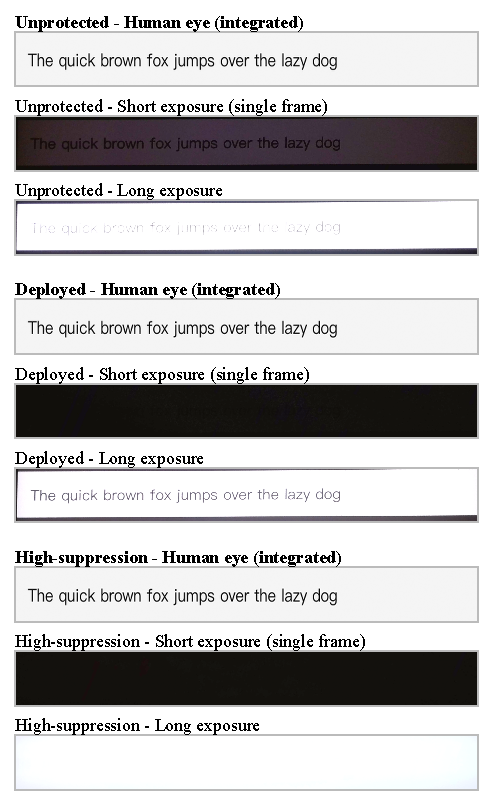
\includegraphics[width=\columnwidth]{figures/real_capture_montage.pdf}
\caption{Real-capture montage at 1.0\,m and $0^{\circ}$. Within each vertically stacked profile group (unprotected, readability-priority, and high-suppression), panels show, from top to bottom, the digital integrated reconstruction, 3.91\,ms short-exposure capture, and 31.25\,ms long-exposure capture. Camera panels are identically cropped from the archived raw camera JPEGs with no geometric correction or brightness gain, so they differ from the geometrically corrected crops used for OCR evaluation. Digital panels use the same $1920\times1080$ black playback canvas and brightness-aligned full-cycle integration for each profile; the readability-priority and high-suppression reconstructions include the recorded $\alpha=0.2$ inversion slot. These digital views are not direct evidence of human readability or visual comfort.}
\label{fig:montage}
\end{figure}

\begin{figure}[!t]
\centering

\includegraphics[width=\columnwidth]{figures/real_capture_bar.pdf}
\caption{Best-of-engine OCR character recovery and exact match for three representative real-capture profiles (unprotected, readability-priority, and high-suppression) under short exposure, long exposure, and a 150-frame video temporal mean, pooled across the 9 tested distance--angle configurations. Lower bars indicate less recovered text. The long-exposure and video bars expose the integration boundary: the readability-priority profile retains substantial recoverable content even when its short-exposure bar is low. Readability-priority sample counts include the disclosed five-item repeat and therefore differ from the other profiles.}
\label{fig:bar_attack}
\end{figure}

\textbf{Per-engine results}: Table~\ref{tab:real_ocr_engine} breaks down pooled short-exposure results by engine; Fig.~\ref{fig:real_engine_ocr} visualizes all six profiles. The engines differ widely in unprotected recovery (Surya 37.1\%, EasyOCR 79.5\%, Tesseract 84.3\%). Under Strong, recovery ranges from 2.1--16.3\%; under readability-priority, 3.2--11.7\%; under high-suppression, 1.8--2.0\%. All three show reduction, but the finding is neither recognizer-agnostic nor preprocessing-agnostic. The metric-wise best-of-engine aggregation is attacker-favorable within this limited set, not an upper bound over optimized or commercial OCR pipelines.

The evaluated engines are open-source conventional OCR systems; commercial OCR APIs such as Google Cloud Vision, Azure AI Vision, or Baidu OCR were not tested and may achieve higher recovery. The three-engine best-of-engine result should therefore be read as an attacker-favorable aggregation within a limited engine set, not as an upper bound over available OCR services.

\begin{table}[!t]
\caption{Real-Capture Short-Exposure OCR: Per-Engine Results (Pooled Across 9 Geometric Conditions)}
\label{tab:real_ocr_engine}
\centering
\footnotesize
\setlength{\tabcolsep}{5.5pt}
\begin{tabular}{llccc}
\toprule
Profile & Engine & Char (\%) & Exact (\%) & N \\
\midrule
\multirow{3}{*}{Original}
 & Surya & 37.1 & 22.8 & 324 \\
 & EasyOCR & 79.5 & 27.8 & 324 \\
 & Tesseract & 84.3 & 47.8 & 324 \\
\midrule
\multirow{3}{*}{Mask only}
 & Surya & 4.2 & 0.3 & 324 \\
 & EasyOCR & 15.6 & 0.0 & 324 \\
 & Tesseract & 3.2 & 0.0 & 324 \\
\midrule
\multirow{3}{*}{Mask + noise}
 & Surya & 11.0 & 2.8 & 324 \\
 & EasyOCR & 18.1 & 0.0 & 324 \\
 & Tesseract & 4.8 & 0.0 & 324 \\
\midrule
\multirow{3}{*}{Strong}
 & Surya & 6.1 & 0.6 & 324 \\
 & EasyOCR & 16.3 & 0.0 & 324 \\
 & Tesseract & 2.1 & 0.0 & 324 \\
\midrule
\multirow{3}{*}{Readability-priority}
 & Surya & 3.2 & 0.4 & 459 \\
 & EasyOCR & 11.7 & 0.0 & 459 \\
 & Tesseract & 3.3 & 0.0 & 459 \\
\midrule
\multirow{3}{*}{High-suppression}
 & Surya & 1.8 & 0.0 & 324 \\
 & EasyOCR & 2.0 & 0.0 & 324 \\
 & Tesseract & 1.9 & 0.0 & 324 \\
\bottomrule
\end{tabular}
\end{table}

\begin{figure}[!t]
\centering
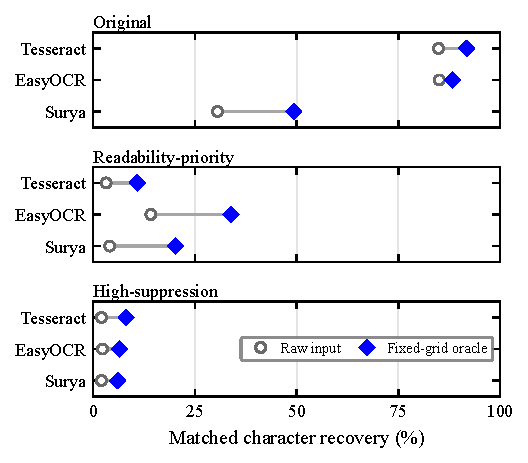
\includegraphics[width=\columnwidth]{figures/real_engine_ocr.pdf}
\caption{Real-capture short-exposure character recovery for three OCR engines across all six profiles in Table~\ref{tab:real_ocr_engine}; error bars are 95\% bootstrap intervals resampled by capture. All three engines are suppressed, but with a limited engine family this cannot be claimed as recognizer-agnostic.}
\label{fig:real_engine_ocr}
\end{figure}

\subsection{Real-Capture VLM Probes}
\label{sec:vlm}

To test whether conventional OCR conclusions extend to stronger recognizers, we applied three commercial VLM endpoints exposed through the SiliconFlow API (Qwen3-VL-32B-Instruct~\cite{b_qwen3vl2025}, Kimi-K2.6, and GLM-4.5V~\cite{b_glm45v2025}) to the same real-capture photographs. This section is a \emph{boundary probe}: if VLMs recover text where conventional OCR fails, the practical scope of the method is confined to conventional OCR short-exposure mitigation.

The probes cover 0$^{\circ}$ on-axis at three distances. The 0.5\,m run includes 156 inputs: 36 unprotected short-exposure baselines, 36 high-suppression short- and long-exposure inputs each, and four aggregate views from 60\,fps video (12 segments each). The 1.0\,m and 1.5\,m runs each include 120 high-suppression inputs: 36 short- and long-exposure inputs each plus four video aggregate types (12 segments each). VLM inputs and the OCR best-of-engine (BoE) reference in Table~\ref{tab:real_vlm} use the same file batch with nominal 3.91/31.25\,ms labels. All VLM calls use raw camera JPEGs. The fixed Tesseract grid in \S\ref{sec:real_capture} does not evaluate VLM input preprocessing; pilot CLAHE enhancement recovered additional text, so raw-JPEG VLM results are not an attack upper bound.

Of 1,188 model requests, 1,133 returned parseable results: 34 failures at 0.5\,m, 21 at 1.0\,m, and none at 1.5\,m. Each table cell reports effective $N$ and is conditional on a parseable response. GLM failures concentrate on mixed, digit, and credential items, so missingness cannot be treated as random. We therefore computed cell-wise lower and upper bounds by assigning every failed call 0 or 100\% recovery. For the GLM 0.5\,m short cell, character recovery is bounded by 61.0--74.9\% and exact recovery by 44.4--58.3\%. Conditional cells are not used to rank models; complete bounds for all cells are archived with the analysis.

We use the failure-free 1.5\,m run as primary cross-model evidence; the 1.0\,m run enters the short-exposure distance sweep as supplementary data. At 1.0\,m, Qwen and Kimi long-exposure exact match are 84.4\% and 74.3\%, and the successful calls from the three models yield 70.0--83.3\% exact match under the 150-frame video mean. GLM long-exposure exact match is only 3.3\% at 1.0\,m versus 58.3\% at 1.5\,m, but content-dependent failures preclude a cross-distance consistency claim. For compactness, Table~\ref{tab:real_vlm} reports only the 150-frame video mean at 0.5\,m; the 1.5\,m run reports all four aggregate views to show view-selection sensitivity.

All calls used SiliconFlow's OpenAI-compatible API. The recorded provider identifiers are \texttt{Qwen/\allowbreak Qwen3-\allowbreak VL-\allowbreak 32B-\allowbreak Instruct}, \texttt{Pro/\allowbreak moonshotai/\allowbreak Kimi-\allowbreak K2.6}, and \texttt{zai-\allowbreak org/\allowbreak GLM-\allowbreak 4.5V}. Qwen3-VL and GLM-4.5V have public technical reports~\cite{b_qwen3vl2025,b_glm45v2025}. For Kimi-K2.6, we use the provider endpoint identifier and the archived request metadata as the reproducibility record, rather than making claims about a separately documented upstream public release. The \texttt{Pro/} prefix in the second identifier is SiliconFlow-specific, and the endpoint accepted image inputs in our archived calls. Decoding temperature is 0 and maximum output is 4,096 tokens. The shared prompt requests only visible text and prohibits guessing; ground truth is not provided. Full prompts, parameters, and per-call outputs are archived. Metrics follow \S\ref{sec:setup} and are pooled at the capture level. Public CET6 documents may inflate recovery through training-data memorization, so synthetic snippets and exact match provide cleaner discriminative evidence.

\textbf{0.5\,m session selection transparency}: The archive preserves an alternative session (\path{real_capture_vlm_d0.5_a0_rerun.json}, timestamp 012715) at the same position whose high-suppression short-exposure inputs are nearly all-black, yielding empty transcriptions and 0\% char/exact across all three models. Table~\ref{tab:real_vlm} uses the 141107 (3.91\,ms) session because it shares the OCR reference batch and its inputs are not black. These are the only two 0.5\,m on-axis VLM sessions, so Qwen's observed short-exposure exact-match outcome ranges from 0/36 captures in the underexposed session to 28/36 captures in the tabled session, not a stable single-session estimate. The adequate-exposure criterion was applied after inspecting two sessions and is therefore a post-hoc selection rule; preserving both sessions and reporting the range makes the exposure sensitivity explicit. The tabled session is the conservative attacker-favorable case, while the alternative is retained as an underexposure diagnostic.

\begin{table*}[!t]
\caption{Real-Capture VLM Probes (0$^{\circ}$ On-Axis; All Rows Except the Original Short Baseline Are High-Suppression). Each VLM Cell Reports Exact Count / Char / $N$ (Recoveries / \% / Effective Calls); Cells with Failures Are Conditional on Parseable Responses. OCR BoE Shows the Same-Batch Three-Engine Best-of-Engine Reference (Exact / Char, \%). The Temporal-Mean Rows Average 150 Short-Exposure Frames; Other Aggregate Views Are Defined in the Text. The 0.5\,m high-suppression short row uses the adequate-exposure attacker-favorable 141107 session; the only alternative 0.5\,m session was underexposed and yielded 0/36 Qwen exact matches.}
\label{tab:real_vlm}
\centering
\footnotesize
\setlength{\tabcolsep}{4.2pt}
\begin{tabular}{llcccc}
\toprule
Distance & Condition & OCR BoE & Qwen3-VL-32B & Kimi-K2.6 & GLM-4.5V \\
\midrule
\multicolumn{6}{l}{\textit{Short-exposure distance sweep}}\\
\midrule
0.5\,m & original short & 58.3~/~92.4 & 30~/~94.5~/~36 & 30~/~95.6~/~36 & 19~/~92.0~/~26 \\
0.5\,m & short & 0.0~/~8.4 & 28~/~91.5~/~36 & 17~/~84.7~/~36 & 16~/~70.8~/~31 \\
1.0\,m & short & 0.0~/~3.6 & 20~/~79.1~/~36 & 14~/~68.6~/~36 & 9~/~47.0~/~33 \\
1.5\,m & short & 0.0~/~6.5 & 17~/~68.9~/~36 & 12~/~61.5~/~36 & 13~/~70.0~/~36 \\
\midrule
\multicolumn{6}{l}{\textit{Key attack views}}\\
\midrule
0.5\,m & long & 0.0~/~2.1 & 28~/~85.7~/~34 & 1~/~7.9~/~36 & 0~/~4.9~/~30 \\
0.5\,m & Video (150-frame mean) & 8.3~/~50.7 & 10~/~94.0~/~12 & 10~/~95.5~/~12 & 7~/~91.8~/~8 \\
1.5\,m & long & 0.0~/~13.2 & 33~/~89.3~/~36 & 32~/~89.9~/~36 & 21~/~62.4~/~36 \\
1.5\,m & Video (single best) & 0.0~/~4.3 & 1~/~24.8~/~12 & 0~/~12.7~/~12 & 0~/~29.8~/~12 \\
1.5\,m & Video (150-frame mean) & 0.0~/~48.4 & 8~/~90.3~/~12 & 8~/~90.3~/~12 & 7~/~88.5~/~12 \\
1.5\,m & Video (window-mean best) & 0.0~/~8.6 & 7~/~89.0~/~12 & 5~/~84.2~/~12 & 8~/~87.2~/~12 \\
1.5\,m & Video (max projection) & 0.0~/~19.0 & 8~/~90.1~/~12 & 7~/~89.2~/~12 & 7~/~88.7~/~12 \\
\bottomrule
\end{tabular}
\end{table*}

\begin{table}[!t]
\caption{0.5\,m High-Suppression Short-Exposure VLM Character Recovery by Content Type. Baseline Column Shows Same-Session Unprotected Original Short Results for Qwen (Kimi/GLM Similar); GLM Had Occasional Call Failures, Parenthesized $N$ Shows Effective Count. At 1.5\,m, CET6 Dense Pages Yield 0\% Char Across All Three Models.}
\label{tab:vlm_content}
\centering
\footnotesize
\setlength{\tabcolsep}{2.8pt}
\begin{tabular}{lcccc}
\toprule
Content type ($N$) & Baseline (\%) & Qwen (\%) & Kimi (\%) & GLM (\%) \\
\midrule
CET6 document (3) & 64.4 & 18.5 & 5.6 & 0.4 \\
Credentials (6) & 97.6 & 97.6 & 88.3 & 77.1~(5) \\
Code snippets (6) & 89.8 & 94.9 & 95.8 & 88.9 \\
Digit strings (6) & 100.0 & 100.0 & 98.6 & 50.0~(4) \\
Mixed content (6) & 100.0 & 100.0 & 92.5 & 98.2~(4) \\
Paragraphs (6) & 100.0 & 99.8 & 81.7 & 66.5 \\
English sentences (3) & 95.3 & 95.3 & 96.9 & 94.6 \\
\bottomrule
\end{tabular}
\end{table}

Table~\ref{tab:real_vlm} presents the pooled VLM probe results: short-exposure rows show distance variation, while long-exposure and video aggregate rows show integration attack boundaries. Table~\ref{tab:vlm_content} breaks down 0.5\,m high-suppression short-exposure character recovery by content type.

\textbf{Key findings}:

\begin{enumerate}
\item \textbf{VLMs bound rather than extend the claim}: On the same 0.5\,m photographs, best-of-engine OCR yields only 8.4\% char / 0\% exact on the high-suppression short-exposure condition, while Qwen3-VL achieves 91.5\% char and exactly recovers 28/36 captures from 12 items. At 1.5\,m, the three models retain 33.3--47.2\% exact / 61.5--70.0\% char. Even with a prompt prohibiting guessing, VLMs recover substantial text from visible fragments. Within this on-axis, high-suppression, three-distance probe, conventional OCR claims therefore do not transfer to VLM attackers; off-axis VLM capture and other protection profiles were not evaluated.

\item \textbf{Failure concentrates on large-font short snippets}: At 0.5\,m, CET6 document pages yield 0.4--18.5\% VLM character recovery, whereas credentials, code, and digit strings yield 50--100\% (Table~\ref{tab:vlm_content}). At 1.5\,m, CET6 pages drop to 0\% across the three models, while digit strings and short sentences remain recoverable. This is consistent with font scale and language priors~\cite{b_shi2023,b_jiang2025}, but the experiment does not isolate either mechanism.

\item \textbf{Attack capability varies across models and conditions}: In the failure-free 1.5\,m session, nominal long-exposure exact recovery ranges from 58.3\% to 91.7\%, with 62.4--89.9\% character recovery. This spread is descriptive and should not be interpreted as a stable model ranking. VLM behavior depends on endpoint version, distance, capture view, and content.

\item \textbf{Sustained video aggregation is a VLM failure boundary}: At 0.5\,m, missingness bounds for the 150-frame mean span 58.3--91.7\% exact and 61.2--95.5\% character recovery across models. All aggregate views come from the same burst and do not represent independent short-duration attacks. In the failure-free 1.5\,m session, the 150-frame mean yields 58.3--66.7\% exact and 88.5--90.3\% character recovery, while single-best-frame exact recovery is 0--8.3\%. The experiment does not determine a minimum recording duration.
\end{enumerate}

The effectiveness claim must therefore be bounded by content and attacker type: the high-suppression profile reduces dense small-text recovery under conventional OCR in this probe, but large-font short snippets (credentials, code, digit strings) remain recoverable when the attacker uses a modern VLM. This negative result repositions the practical scope from ``blocking arbitrary machine screen-reading'' to ``reducing conventional OCR short-exposure batch recovery,'' and identifies VLM-aware display protection as an open problem. Countermeasure directions are discussed in \S\ref{sec:vlm_defense}. The section covers a single camera at 0$^{\circ}$ on-axis, one profile, three commercial API models, and only 12 video segments per cell; numbers are descriptive boundary probes, not full cross-geometry or cross-model-version evaluation.

% Defined here for source locality with the real-capture protocol, but emitted
% after all attack experiments so the evaluation narrative remains continuous.
\long\def\deferreduserstudy{
% ----------------------------------------------------------
\subsection{User Experience Study}
\label{sec:user_study}

To evaluate the impact of the protected display on human readability and visual comfort, we designed a web-based user study.

\textbf{Equipment and environment protocol}: The same 240\,Hz display as in \S\ref{sec:setup}. The formal study version sets a hard measured refresh-rate threshold of $\geq$200\,Hz to ensure the fixed $n=4$ basic subframe cycle rate $f_r/n\geq50$\,Hz; below this threshold participation is blocked rather than silently reducing $n$. The 144--199\,Hz adaptive path is available only for an explicitly labeled demonstration mode, and its sessions are excluded from analysis by default. Before each participant begins, the experimenter confirms fixed display brightness, disabled auto-brightness/power-saving and variable refresh rate, unified browser fullscreen, closed high-load background processes, and an approximate 60\,cm viewing distance. Refresh rate is re-measured after any display-mode change.

The browser records actual frame intervals in each trial's \path{requestAnimationFrame} loop; if the interval between adjacent callbacks exceeds 1.5$\times$ the expected interval computed from the pre-trial measured refresh rate, a dropped-frame event is logged, along with estimated drop count, drop rate, mean/max frame intervals, observed refresh rate, basic subframe cycle rate, and full cycle rate with inversion frame. This recording reflects only browser presentation cadence and cannot substitute for panel scanning or photometric measurement.

\textbf{Ethics and safety}: The planned study involves minimal-risk human-subjects research, and no participant data have been collected. Before recruitment, the authors will obtain and document a written approval, exemption, or waiver determination from the competent institutional or departmental authority; formal data collection will not begin without that determination. Participants must separately check informed consent and photosensitivity screening: the page explicitly states that the masked display involves rapid temporal modulation, that participants should stop immediately upon experiencing discomfort, eye fatigue, dizziness, nausea, or headache, and that they may withdraw unconditionally at any time. Individuals who self-report a history of photosensitive epilepsy or sensitivity to flicker are not permitted to proceed. The system records consent timestamps and screening pass flags. The implementation applies a conservative $f_r/n\geq50$\,Hz operating floor, but this engineering gate is not an ethical or clinical safety determination. At $n=4$ on a 240\,Hz panel the basic cycle rate is 60\,Hz; the inversion frame reduces the full cycle frequency to $f_r/(n+1)=48$\,Hz, and the implementation separately logs warnings and actual timing. Registration information (student ID, name) is used only for participation management; analysis and publication use only de-identified data. Age and gender are optional demographic fields.

\textbf{Task design}: Each participant first completes one 12-second, unscored unmasked Canvas typing warm-up, views a 10-second, unscored readability-priority full-mask preview, and then completes an 8-second, unscored typing practice under the same readability-priority mask. This sequence separates initial stimulus and input adaptation from the four subsequent 20-second scored trials (within-subjects design). On every typing screen, including warm-up, practice, and scored trials, the stimulus Canvas is visible and its player has started before the participant clicks ``Start.'' Clicking ``Start'' triggers a 5-second countdown while the input remains disabled; the timed typing interval and input availability begin only when the countdown ends. The same pre-start viewing procedure applies to both control and masked conditions.

The two conditions are each repeated twice. The experimenter's continuously assigned zero-based sequence number $k$ selects ABBA or BAAB order to counterbalance practice and fatigue: (A)~\textbf{original text} (control), displayed as unmasked Canvas with $n=1$; (B)~\textbf{masked text}, using the readability-priority configuration: $n=4$, mask+noise, strong anti-OCR ($\alpha_s=0.10$, $\alpha_g=0.12$, 6 cycles) + weak inversion ($\alpha=0.2$). The typing order index is $k\bmod2$, and the subjective-rating Latin-square row is $\lfloor k/2\rfloor\bmod6$. Every consecutive 12~participants therefore cover all $2\times6$ joint assignments. Formal sessions enforce a uniqueness constraint on $k$, and the backend recomputes and verifies both order indices.

Both conditions are rendered by the same \texttt{render\allowbreak Source\allowbreak Canvas} path, with identical dark background, light text, canvas size, 23\,px bold font, and color. The sole processing difference is the temporal protection pipeline, avoiding polarity and font-weight confounds. Here ``cycles'' means that the web implementation rotates through six distinct mask, noise, and stripe instances before repeating. This web-playback-specific setting shares $\alpha_s$ and $\alpha_g$ with the real-capture configuration in \S\ref{sec:method} and avoids repeatedly integrating one fixed overlay pattern.

Scoring no longer compares characters position-by-position but aligns the full transcription against the optimal target prefix using Levenshtein minimum string distance (MSD)~\cite{b_soukoreff2003}; untyped target suffix does not count as error. The alignment yields accuracy, characters per minute (CPM), and words per minute (WPM), along with edit distance, aligned prefix length, and scoring version. First-keystroke latency is defined from the end of the 5-second countdown, when the input is enabled and the scored timer starts, to the first input event that makes the transcription non-empty. Analysis first averages each participant's two trials per condition, then performs within-subject paired comparison.

\textbf{Subjective ratings}: After the typing trials, participants rate 6~conditions on the three 1--5 Likert items displayed by the interface: readability (1 = difficult to read, 5 = very clear), stability (stored in the \texttt{flicker} field; 1 = strong flicker, 5 = no perceptible flicker), and immediate visual comfort (\texttt{fatigue}; 1 = very uncomfortable, 5 = very comfortable). Higher values therefore indicate a better outcome on every item. Conditions include the unmasked original anchor, $n\in\{2,3,4\}$ mask+noise, $n=4$ mask-only, and the same $n=4$ readability-priority full configuration (mask+noise+strong anti-OCR+weak inversion) used in the typing task. The first three masking levels all achieve $\geq$60\,Hz real temporal playback on a 240\,Hz panel; the originally planned $n=8$ would yield 30\,Hz and trigger static fallback, so it is not included as a temporal ablation. The six conditions are presented in a 6th-order balanced Latin square; each condition must be viewed for at least 10~seconds before submission is enabled, with viewing start/end times and duration recorded. The unmasked anchor is also an attention/scale-interpretation aid but is not mechanically excluded by a ``must rate 5'' rule. This study does not include the high-suppression profile; assessment of its visible stripes and grain's acceptability is left to future work (see \S\ref{sec:discussion}).

\textbf{Sample size and analysis plan}: A minimum of $N=24$ participants is planned, a number within the range required for paired effect sizes of $d_z\approx0.6$--$0.8$ at 80\% power, and exactly covering two rounds of the 12-person joint order assignment. Pre-registered exclusion criteria are debug/demo sessions, incomplete four typing or six rating records, measured refresh rate below 200\,Hz, any typing trial with fewer than 5 attempted characters, control mean accuracy below 50\%, masked trials not in temporal mode, any trial with observed basic cycle rate below 50\,Hz, or minimum-view straight-line ratings. The last criterion is defined as all six rating rows having a recorded viewing duration no greater than 11~seconds (a 1-second tolerance above the 10-second submission gate) and, within every row, identical scores on all three items. WPM, CPM, accuracy, attempted characters, and first-keystroke latency are first averaged within each participant by condition; speed metrics must be interpreted jointly with accuracy to avoid misinterpreting fast input under low accuracy as performance improvement. Paired differences are tested using paired $t$-tests when the pre-specified Shapiro test is passed, otherwise Wilcoxon signed-rank tests, with effect sizes and participant-level bootstrap 95\% confidence intervals reported. Likert data are analyzed per dimension using Friedman tests with Holm-corrected post-hoc pairwise Wilcoxon tests. Analysis scripts generate de-identified participant means, JSON audit reports, and two \LaTeX\ tables directly from the formal database \texttt{study\_formal.db}.

% NOTE: All "XX" marks and "--" table cells below are pending data placeholders.
% After the study, run webstudy/analyze_study.py; its analysis_output/typing_table.tex
% and ratings_table.tex rows map one-to-one onto Tables \ref{tab:study_typing} and
% \ref{tab:study_ratings}, and experiments/paper_figures/make_all.py regenerates
% Figs. \ref{fig:study_typing} and \ref{fig:study_ratings} from the same output.
\textbf{Participants}: XX volunteers were recruited; XX sessions met all pre-registered inclusion criteria and entered analysis (XX excluded; per-criterion audit counts accompany the released analysis output). Optional demographics for the included sample: XX of XX reported age (median XX years, range XX--XX) and XX reported gender (XX women, XX men). All formal sessions ran on the 240\,Hz laboratory display with a measured refresh rate of at least 200\,Hz.

\begin{table}[!t]
\caption{Typing Task: Within-Subject Comparison of the Control and Readability-Priority Masked Conditions ($N=$ XX; Participant Means Over Two Trials per Condition; $\Delta$ = Masked $-$ Control With Participant-Level Bootstrap 95\% CI). Per Metric, a Paired $t$-Test Is Used When the Pre-Specified Shapiro Test Passes (Effect Size Cohen's $d_z$), Otherwise a Wilcoxon Signed-Rank Test (Effect Size Rank-Biserial $r_{rb}$); Test Statistics Are Reported in the Text}
\label{tab:study_typing}
\centering
\footnotesize
\setlength{\tabcolsep}{4pt}
\begin{tabular}{lccc}
\toprule
Metric & Control & Masked & $\Delta$ [95\% CI] \\
\midrule
Accuracy (\%) & -- & -- & -- [--, --] \\
WPM & -- & -- & -- [--, --] \\
CPM & -- & -- & -- [--, --] \\
Attempted chars & -- & -- & -- [--, --] \\
First-key latency (ms) & -- & -- & -- [--, --] \\
\bottomrule
\end{tabular}
\end{table}

\begin{table}[!t]
\caption{Subjective Ratings for the Six Display Conditions ($N=$ XX; 1--5 Likert, Higher Is Better; Mean $\pm$ SD). Stability Is the Inverse-Flicker Item and Comfort the Immediate Visual Comfort Item (\S\ref{sec:user_study}); Friedman and Holm-Corrected Pairwise Wilcoxon Statistics Are Reported in the Text}
\label{tab:study_ratings}
\centering
\footnotesize
\setlength{\tabcolsep}{4pt}
\begin{tabular}{lccc}
\toprule
Condition & Readability & Stability & Comfort \\
\midrule
Unmasked anchor & -- & -- & -- \\
$n{=}2$ mask+noise & -- & -- & -- \\
$n{=}3$ mask+noise & -- & -- & -- \\
$n{=}4$ mask+noise & -- & -- & -- \\
$n{=}4$ mask-only & -- & -- & -- \\
Readability-priority full ($n{=}4$) & -- & -- & -- \\
\bottomrule
\end{tabular}
\end{table}

\textbf{Results}: Table~\ref{tab:study_typing} and Fig.~\ref{fig:study_typing} summarize the typing task. Relative to the control condition, the readability-priority full configuration changed mean accuracy by XX percentage points (95\% CI [XX, XX], $p=$ XX, effect size XX), WPM by XX (95\% CI [XX, XX], $p=$ XX, effect size XX), and first-keystroke latency by XX\,ms (95\% CI [XX, XX], $p=$ XX, effect size XX); CPM and attempted characters gave $p=$ XX and XX, respectively. Table~\ref{tab:study_ratings} and Fig.~\ref{fig:study_ratings} summarize the subjective ratings: Friedman tests yielded $\chi^2=$ XX ($p=$ XX) for readability, $\chi^2=$ XX ($p=$ XX) for stability, and $\chi^2=$ XX ($p=$ XX) for immediate visual comfort; Holm-corrected pairwise comparisons between the readability-priority full configuration and the unmasked anchor gave $p=$ XX, XX, and XX on the three items, respectively.

\begin{figure}[!t]
\centering

\includegraphics[width=\columnwidth]{figures/study_typing_paired.pdf}
\caption{Within-subject typing performance under the control and readability-priority masked conditions: each gray line is one participant (mean of two trials per condition); markers show group means with participant-level bootstrap 95\% confidence intervals. Panels show transcription accuracy, words per minute, and first-keystroke latency.}
\label{fig:study_typing}
\end{figure}

\begin{figure}[!t]
\centering

\includegraphics[width=\columnwidth]{figures/study_ratings_likert.pdf}
\caption{Mean 1--5 Likert ratings (error bars: SD) for readability, stability, and immediate visual comfort across the six rated display conditions, ordered from the unmasked anchor to the readability-priority full configuration. Higher is better on every item.}
\label{fig:study_ratings}
\end{figure}

}

% ----------------------------------------------------------
\subsection{Supplementary Detection and Tracking Diagnostics}

Object-detection and tracking diagnostics are reported in the supplementary material rather than the main evidence chain. They use one real-capture position, a limited COCO subset, still-frame MOT captures, and approximate simulation metrics, so they are diagnostic stress tests but do not extend the primary conventional-OCR claim. The normalized cross-task summary figure is omitted from the main paper because OCR character recovery, mAP, higher-order tracking accuracy (HOTA), and identification F1 (IDF1) are not commensurate measurements.

% ----------------------------------------------------------
\subsection{Software Simulation Supplementary Experiments}

This section uses software simulation to address two questions: (1)~what is the machine readability of one protected subframe obtained after the application renderer? (2)~what is recovery under zero camera noise and perfect alignment? The 0--2.6\% results characterize only a capture point after masking that returns one protected subframe. Operating-system screenshot APIs may capture before masking, after compositing, or across recorded frames; those paths were not tested. Malware that intercepts the original frame or recording that accumulates a full cycle bypasses the method. We therefore make no general ``anti-screenshot'' claim.

\subsubsection{Synthetic Single-Subframe OCR}
Using Tesseract~\cite{b_smith2007}, EasyOCR~\cite{b_easyocr2020}, and Surya~\cite{b_surya2024} on 120 synthetic samples, character recovery drops from 94.0--97.0\% to 0--2.6\% across three engines (Table~\ref{tab:ocr_corpus}). The result covers the current corpus, parameters, and engine set; stratified breakdowns can check category trends but are insufficient to prove effectiveness across all languages, layouts, or recognizers.

\begin{table}[!t]
\caption{Synthetic Single-Subframe OCR: Three-Engine Character Recovery (120 Samples, $n=4$, $\varepsilon=8/255$)}
\label{tab:ocr_corpus}
\centering
\footnotesize
\begin{tabular}{lccc}
\toprule
OCR engine & Original frame & Single subframe & Reduction \\
\midrule
Tesseract & 94.0\% & 0.0\% & 94.0\% \\
EasyOCR & 94.1\% & 0.0\% & 94.1\% \\
Surya & 97.0\% & 2.6\% & 94.4\% \\
\bottomrule
\end{tabular}
\end{table}

\begin{figure}[!t]
\centering

\includegraphics[width=\columnwidth]{figures/multiengine_ocr.pdf}
\caption{Character recovery for three OCR engines on original frames and single protected subframes; error bars are 95\% bootstrap intervals resampled by corpus sample.}
\label{fig:multiengine_ocr}
\end{figure}

Fig.~\ref{fig:multiengine_ocr} visualizes these results. Single-subframe recovery does not exceed 2.6\% for any engine, confirming the finding is not driven by one recognizer. Broader generalization requires additional engines and corpora.

\subsubsection{Theoretical Security Boundary}
\label{sec:security_frontier}
When an attacker accumulates registered frames covering a full cycle, complementary subframes can be re-summed in the ideal linear model of~(\ref{eq:noise_complement}). The archived per-sample strongest digital attack recovers 95.2\%; pure full-cycle temporal averaging recovers 94.3\%. This is a reconstruction boundary of the evaluated linear decomposition, not a formal information-theoretic theorem. The high-suppression profile still yields 47.9\% pooled recovery under the 150-frame mean and 53.9\% after excluding the underexposed position. Character recovery need not scale with the illuminated-pixel fraction because recognition also depends on content and the physical imaging path.

\begin{table}[!t]
\caption{Archived Digital Reconstruction Boundary (Tesseract)}
\label{tab:digital_boundary}
\centering
\footnotesize
\setlength{\tabcolsep}{3pt}
\begin{tabular}{lrrrrr}
\toprule
Setting & $N$ & Char. & Exact & SSIM & $\Delta E_{00}$ \\
\midrule
Base: cycle mean & 120 & 94.3\% & 85.8\% & -- & -- \\
Base: per-sample strongest & 120 & 95.2\% & 91.7\% & -- & -- \\
Readability: cycle mean & 16 & 87.9\% & 50.0\% & 0.948 & 1.46 \\
High: cycle mean & 16 & 56.6\% & 6.3\% & 0.764 & 4.87 \\
High: inversion slot & 16 & 93.0\% & 81.2\% & -- & -- \\
\bottomrule
\end{tabular}
\vspace{1mm}

\raggedright\scriptsize The 120-sample base attack and 16-sample profile ablation are separate archived digital evaluations. ``Per-sample strongest'' selects the best result among seven prespecified reconstructions for each sample. Profile SSIM and $\Delta E_{00}$ describe full-cycle reconstruction quality, not physical or user-perceived quality.
\end{table}

Additional software-proxy baseline, parameter-sweep, detection, and tracking diagnostics are preserved outside the main evidence chain. They are not used as main-text evidence because their physical conditions, user-experience costs, and metrics are not matched to the real-capture OCR estimand.

\deferreduserstudy

%% ============================================================
%% VI. DISCUSSION
%% ============================================================
\section{Discussion}
\label{sec:discussion}

\subsection{Evidence Hierarchy and Claim Scope}

The most directly supported conclusion is a fixed-condition observation. At the common nominal setting on one S600 link, the evaluated profiles reduce mean raw-input recovery for three open-source OCR engines. A fixed Tesseract preprocessing grid recovers more text, particularly for high-suppression, and prevents treating raw inputs as an attack upper bound. This is not an exposure interval, a general anti-photography claim, or evidence against an optimized attacker. The unbalanced corpus, single webcam, fixed profile order, and missing luminance-matched controls prevent cross-device or mechanism-isolation inference. VLM, integration, and simulation results define boundaries rather than extend the primary claim. The passive baselines are software proxies and do not establish superiority over physical filters or prior temporal-display systems.

\subsection{The Mathematical Tension of Linear Integration}

The scheme exploits a difference between human temporal perception and a short camera exposure. Its mathematical boundary, however, is defined in an ideal linear display--camera radiance model rather than by treating human vision as a linear summation operator. In that model, complementary subframes can be re-summed to recover the original ($\sum\mathbf{I}_k = \mathbf{I}$), so a camera that accumulates a registered full cycle defeats the linear decomposition. Research on VLM adversarial robustness~\cite{b_jiang2025} further shows that large models extract partial semantic information from perturbed images; the probes in \S\ref{sec:vlm} confirm this. VLMs recover large-font content from single short-exposure photographs and obtain stronger signals from the 150-frame video mean and long-exposure views. The archived digital evaluation reaches 95.2\% under the per-sample strongest attack across all evaluated reconstructions; pure full-cycle temporal-mean recovery reaches 94.3\% (\S\ref{sec:security_frontier}).

\subsection{Physical-Layer Confounds and the Simulation-to-Real Gap}

The simulation-to-real gap is compatible with several physical-layer effects, but none was isolated by the current design.

\textbf{Direction 1: real short-exposure recovery exceeds simulation (favoring the attacker).} Simulated single-subframe OCR yields 0--2.6\% character recovery (Table~\ref{tab:ocr_corpus}), whereas real-capture short-exposure recovery under comparable masking is 19.2\% (mask-only, Table~\ref{tab:real_ocr_full_pool}). Two physical effects could contribute. First, rolling-shutter row mixing can make different rows sample different display phases, although the S600 readout time and phase were not measured. Second, LCD response transitions can blend adjacent subframes; the AOC 24G51Z's specified 1\,ms GtG already occupies about 24\% of a 4.17\,ms slot. Actual gray-level transitions may differ from the nominal GtG specification. The real-capture measurements include both effects, but this experiment does not identify their separate contributions. The simulation is therefore an idealized single-subframe reference, not a physical lower bound.

\textbf{Direction 2: real integration recovery is lower than simulation.} The per-sample strongest digital attack recovers 95.2\% (\S\ref{sec:security_frontier}), whereas the real 150-frame mean yields 71.1\% for readability-priority and 47.9\% for high-suppression. The common-setting values are 79.7\% and 53.9\%. ISP processing, moir\'{e}, blur, and imperfect registration are plausible contributors, but the archive does not identify their presence or magnitude. A purpose-built integration attack could therefore narrow the observed gap.

The simulation and physical experiments therefore answer different questions. Simulation evaluates an idealized single-subframe transform; physical recovery measures the entire archived display--camera pipeline with unresolved confounds.

\subsection{Role and Cost of the Exploratory High-Suppression Profile}

The exploratory high-suppression profile breaks strict completeness through stripe and glyph perturbations and is associated with lower integration recovery. Its digital full-cycle SSIM is 0.764 versus 0.948 for readability-priority, while $\Delta E_{00}$ is 4.87 versus 1.46 (Table~\ref{tab:digital_boundary}). The same digital ablation exposes a direct single-slot failure: after contrast stretching, the inversion frame recovers 93.0\% character accuracy on average and yields 81.2\% exact match. This 93.0\% best-observed digital recovery is the profile's strongest observed digital attack, so the 56.6\% temporal-average result is not a worst-case security bound. Physical capture phase was uncontrolled, and the archive cannot establish worst-phase behavior. In the common-setting pool, high-suppression reaches 5.6\% short-exposure character recovery and 53.9\% under the 150-frame mean. It misses the descriptive $<5\%$ target and only mitigates integration leakage. User acceptance remains untested.

This profile split is central to interpretation. Readability-priority is the only profile connected to the planned comfort study, but it is weaker under explicit-field and integration attacks. High-suppression lowers observed recovery in several views, but its exploitable inversion slot and missing usability evidence preclude a general security claim. The manuscript therefore supports a feasibility niche, not a deployment recommendation.

\subsection{VLM Attackers and Countermeasure Directions}
\label{sec:vlm_defense}

Observed VLM failures concentrate on large-font short snippets (\S\ref{sec:vlm}), while temporal averaging supplies a stronger signal. This pattern is consistent with retained glyph contours and language-prior completion, but the experiment does not isolate either mechanism. We retain the result because it constrains the method's scope: conventional-OCR reduction does not imply VLM resistance. Three unvalidated hypotheses follow: font-size-adaptive granularity, glyph decoys, and field-level rendering policies. Complementary decoys would still cancel under ideal full-cycle integration, and none of these ideas has been physically validated. The practical objective should therefore be framed as increasing attack cost, not making visible information irrecoverable.

\subsection{Sustained Video Attacker}

The evaluated video attack does not establish a four-frame bypass. The capture pipeline records 150 short-exposure frames at nominal 60\,fps, and the reported temporal-mean image averages the complete burst, corresponding to approximately 2.5\,s of nominal capture. This attack does not require the mask seed, phase, or precise frame selection because sustained averaging accumulates multiple display cycles. Its pooled recovery is 71.1\% for the readability-priority profile and 47.9\% for high-suppression, rising to 79.7\% and 53.9\% after excluding the underexposed position. The archive also contains aggregate views selected from the same full burst, but they do not establish recovery from an independently acquired short window. A duration-versus-recovery curve and pre-specified short-window analysis remain unevaluated. The single-shot scope should therefore be distinguished from the measured sustained-recording boundary without assigning an unsupported minimum bypass duration.

\subsection{Deployment Path}

Real-world deployment would require driver-level framebuffer injection, panel/backlight coordination, and verified timing. These steps introduce color management, luminance saturation, frame drops, and synchronization errors. Readability-priority already retains 17.7\% explicit-field recovery under the matched short-exposure analysis and high character recovery under integration attacks. Credentials should therefore not rely on this profile alone. Candidate field-level mitigations require separate readability, exposure, video, and VLM evaluation.

\subsection{Required Confirmatory Physical Protocol}

A confirmatory collection should randomize profile order within each content--geometry block and record wall-clock batch identifiers. It should lock and log exposure mode, gain, white balance, focus, codec, display brightness, and ambient illuminance. A photodiode or high-speed sensor should measure slot timing and display luminance. Each temporal profile should be paired with static controls matched for time-averaged luminance and overlay appearance. Hardware triggering should sweep exposure start across the complete $n+1$ slot cycle, including the inversion slot, with preregistered phase bins and repeats. These controls would separate profile association from time drift, luminance, static overlays, panel response, and capture phase. Until such data exist, the present archive cannot support causal or worst-phase claims.

\subsection{Ethics Statement}

This research is defensive in nature, aiming to protect screen content from unauthorized photography. The attack analysis (\S\ref{sec:security_frontier}) is intended for honest assessment of security boundaries, not as an attack guide. The planned user study would involve human subjects in minimal-risk research; no participant data have been collected. Recruitment will begin only after the competent institutional or departmental authority issues a written approval, exemption, or waiver determination. The protocol specifies informed consent, photosensitivity screening, and voluntary withdrawal as described in \S\ref{sec:user_study}.

\subsection{Limitations}

\begin{enumerate}
\item The user study (\S\ref{sec:user_study}) is a protocol, not completed evidence: no participant data exist yet, so the readability-priority profile's usability remains unvalidated. Even when conducted in a controlled 240\,Hz laboratory, external validity will require broader participant samples and display conditions.
\item Immediate visual comfort is a single-item scale measured after short exposure and does not extend to long-term fatigue or clinical visual discomfort.
\item The PoC is application-layer only, without OS drivers or hardware backlight. Luminance, HDR, and color-difference conclusions come from digital models, lacking photometric or panel-response measurements. Actual playback slot timing was not verified with a photodiode, high-speed camera, or oscilloscope. OS compositor jitter, VSync mismatch, and dropped frames can shift subframe boundaries unpredictably; if a short-exposure window straddles the intended slot edge, the camera captures cross-slot content and real recovery may exceed the values reported here. Because the experiment lacks a luminance-matched static control and matched noise-off enhanced profiles, it cannot separate temporal sparsity, duty-cycle luminance, static overlays, panel response, camera exposure, and ISP processing as mechanisms.
\item Real-capture OCR used one S600 UVC webcam. Ambient illuminance, display luminance, sensor gain, auto-exposure semantics, white-balance state, and focus state were not preserved. Profile order was fixed rather than randomized. Time, batch, and automatic-camera behavior may therefore confound profile or geometry comparisons, but their direction and magnitude cannot be reconstructed. Repeated content and capture-resampling summaries do not substitute for cross-device replication.
\item Real-capture detection used 150 COCO images at a single position; tracking used 450 still-frame captures from one MOT17 sequence, not continuous video. Simulated detection used 8~images with approximate metrics.
\item VLM evaluation covers one camera, 0$^{\circ}$ on-axis, one profile, and three commercial API models (12 video segments per cell). Models may update over time. Public document content may inflate recovery via training-data memorization. We did not evaluate multi-cycle adaptive reconstruction, rolling-shutter phase search, or pre-masking malware interception. Full-cycle integration remains a reconstruction boundary of the evaluated linear design.
\item Conventional OCR evaluation covers Surya, EasyOCR, and Tesseract but no commercial OCR API. Best-of-engine over these three systems is attacker-favorable within the evaluated set, yet Google Cloud Vision, Azure AI Vision, Baidu OCR, or future recognizers may obtain higher recovery.
\item Baseline comparisons use unmatched software proxies rather than physically tested privacy filters or prior temporal-display systems. They contextualize the observed trade-off but do not establish comparative superiority over those alternatives.
\item Readability-priority is not suitable as the sole layer for sensitive fields: matched short-exposure field-micro recovery is 17.7\%, and integration/VLM attacks recover substantially more content. Independent access controls remain necessary.
\item The 12-item corpus is mixed rather than all-English/ASCII: the CET6 page and two mixed-language snippets contain Chinese characters. It is too small and selectively constructed to support script-level comparisons; dedicated non-Latin evaluation remains future work.
\end{enumerate}


%% ============================================================
%% VII. CONCLUSION
%% ============================================================
\section{Conclusion}
\label{sec:conclusion}

We measured profile-level display processing at one nominal UVC control setting. Across 8 common-setting geometries, the same 288 matched units per profile yield 94.5\% mean recovery unprotected, 17.8\% for readability-priority, and 5.6\% for high-suppression. Paired content-cluster contrasts are 76.7 percentage points ([74.3, 79.2]) and 88.9 points ([85.5, 91.9]). These results support a fixed-link association for three open-source OCR engines. They do not establish an exposure interval, a causal temporal mechanism, or worst-phase robustness. Readability-priority retains 17.7\% matched field-micro recovery and 95.0\% P99 character recovery, while high-suppression misses its descriptive $<5\%$ target.

The bypass evidence is equally restrictive. A 150-frame temporal mean recovers 71.1\% character for readability-priority and 47.9\% for high-suppression; the common-setting values are 79.7\% and 53.9\%. In the full 9-geometry sensitivity pool, long-exposure recovery at the nominal control setting is 60.9\% for readability-priority versus 47.3\% unprotected. On-axis VLM probes also recover substantial large-font content. The fixed Tesseract grid evaluates five transforms, but optimized preprocessing and transformed EasyOCR/Surya inputs remain outside the supported condition.

The study therefore contributes a bounded physical measurement and explicit failure constraints, not a deployable anti-camera defense. The next decisive experiments are randomized collection, measured phase and luminance controls, an exposure--recovery curve, usability testing, and cross-device replication.

%% ============================================================
%% DATA AND CODE AVAILABILITY
%% ============================================================
\section*{Data and Code Availability}

The software, experimental configurations, de-identified per-sample OCR results, VLM records, and analysis scripts are maintained at \url{https://github.com/docandyc/privacy-display}. The repository is currently mutable and is not presented as an immutable submission artifact. A release tag, commit hash, or archival DOI must be inserted in the final submission package before reproducibility claims rely on a frozen version. VLM records include endpoint identifiers, timestamps, prompts, decoding parameters, input hashes or paths, parse status, and raw outputs. The archived identifiers \texttt{capture\_hardened} and \texttt{vlm} both denote high-suppression. If the user study is conducted, identifiable registration data will not be released; only de-identified results and audits will be public.

%% ============================================================
%% ACKNOWLEDGMENT
%% ============================================================
\section*{Acknowledgment}
\TODO{Acknowledgment to be filled.}

OpenAI Codex~\cite{b_openai_codex2026} assisted with analysis-script development, consistency checks, and English revision of the Abstract, Introduction, Experimental Evaluation, Discussion, and Conclusion. The authors specified the scientific decisions, verified generated analyses against archived data, reviewed all retained text and code, and remain responsible for the manuscript.


%% ============================================================
%% REFERENCES
%% ============================================================
\bibliographystyle{IEEEtran}
\bibliography{refs}
\EOD

\vfill

\end{document}
